\documentclass[11pt,a4paper]{article}
\usepackage[T1]{fontenc}
\usepackage{lmodern,amsmath,amssymb,amsthm,booktabs,microtype,graphicx}
\usepackage[margin=24mm]{geometry}
\usepackage[colorlinks=true,urlcolor=blue,linkcolor=blue]{hyperref}
\newcommand{\Js}{\mathcal J_s}
\newcommand{\av}[1]{\langle #1\rangle}
\DeclareMathOperator{\sech}{sech}
\title{The cubic singlet two-point kernel\\An all-order endpoint-orbit reduction}
\author{Alan Day \and Chengheng\thanks{AI research assistant (OpenAI).}}
\date{Local research note --- 6 November 2026}
\begin{document}\maketitle
\begin{abstract}
The cubic derivative singlet constructed in our preceding note obeys
the $q^3$ probe rule at every fixed two-arc degree. We prove this by
reducing arbitrary chord diagrams to 177 endpoint templates and
verifying their finite polynomial identities with two independent
enumerations. Every template with fewer than three bridges between
the insertions cancels. The surviving three bridges give the known
$q$-Mehler kernel, now for this particular same-coupling composite.
The normalized real-time function tends to
$\sech^6(2\mathcal J_s t)$ in the subsequent small-coupling limit.
\end{abstract}
\section{The operator and the result}
Use standard CAR and the full annealed trace
$\av{Y}=\mathbb E_J2^{-N}\operatorname{Tr}Y$ at
$\beta=\mu_{\rm chem}=0$. Let $H=H_s$ be the Hermitian complex
$p$-creation/$p$-annihilation Hamiltonian, with overlapping index
sets included. Take double scaling first:
\[
 N,p\to\infty,\quad \lambda=p^2/N>0,\quad q=e^{-4\lambda},
 \qquad \sigma^2=\av{H^2}=\Js^2/\lambda .
\]
With $L=[H,\cdot]$, define
\[
 A=\sum_i(Lc_i)^\dagger Lc_i,\qquad
 T_3=\tfrac12\left(\sum_i c_i^\dagger L^3c_i+\mathrm{h.c.}\right).
\]
The finite-$N$ identity $M_3=T_3+\tfrac32LA$ removes the already
known time descendant. Write $\mathcal W_3$ for third Gaussian
\emph{coupling} chaos, and set
\begin{gather}
 R=\mathcal W_3(T_3-a\{H,A\}/2-bH^3),\\
 a=-\frac{(1-q)^2}{1+q^2},\qquad
 b=\frac{2\lambda(1-q)(1+q^3)}{(1+q^2)(1+q+q^2)}.
\end{gather}
Its double-scaled norm is $\av{R^2}=\sigma^6V$, where
\begin{equation}
 V=\frac{4\lambda(1+q)[1-q^3+4\lambda q^2(2q^2-q+2)]}
 {(1+q^2)(1+q+q^2)}>0.                                \label{V}
\end{equation}
For every fixed $u,v\ge0$ we establish
\begin{equation}
 \boxed{\frac{\av{RH^uRH^v}_{\rm DS}}{\sigma^{6+u+v}}
       =V P_{uv}(q,q^3).}                              \label{all}
\end{equation}
Here $P_{uv}(q,r)$ is the standard unit-variance probe moment:
sum over Hamiltonian pairings with weight $q$ per Hamiltonian
crossing and $r$ per crossing of the probe. Odd $u+v$ gives zero.

\newpage
\section{The marked rule and a finite endpoint problem}
Let $K_{ij}$ count normal-order contractions between factors $i,j$
of a three-factor word. The body-rank identity in the preceding
note gives
\[
 T_3=K_{13}-\tfrac12(K_{12}+K_{23}),\qquad
 \{H,A\}/2=\tfrac12(K_{12}+K_{23}).
\]
Thus the insertion $R$ has marks
\begin{equation}
 (12,23,13):\quad
 \left(-\frac{q}{1+q^2},-\frac{q}{1+q^2},1\right),
 \qquad\hbox{and unmarked coefficient }-b.             \label{marks}
\end{equation}
Ordinary Gaussian Wick ordering deletes pairings internal to each
three-slot insertion. It does not forbid a slot from pairing to an
external Hamiltonian.

For a remaining pairing $\pi$, let $c(\pi)$ be its crossing number.
The fixed-word Poisson-overlap rule derived from the local CAR
determinant assigns to two marks the factor
\begin{equation}
 q^{c(\pi)}(\lambda\delta+\lambda^2\alpha\beta).
\end{equation}
Single marks carry $\lambda\alpha$ or $\lambda\beta$, and no mark
carries one. The two-by-two minors give a particularly simple form.
For a mark joining positions $i<j$ within one contiguous insertion,
\begin{equation}
 \alpha_{ij}=2-4\,\mathbf1_{\text{incident chords cross}}. \label{alpha}
\end{equation}
For marks $(i,j)$ and $(k,l)$ in the first and second insertions,
\begin{equation}
 \delta_{ij,kl}
 =4\,\mathbf1_{\pi(i)=l,\ \pi(j)=k}.                   \label{delta}
\end{equation}
For example, differentiating the minor on indices $j,\pi(i)$
gives
$-2\operatorname{sgn}(\pi(j)-\pi(i))/(s_i s_j)$,
$s_i=\operatorname{sgn}(\pi(i)-i)$, which is (\ref{alpha}).
The double derivative can occur only in one minor with two marked
off-diagonal entries, giving (\ref{delta}).

To keep the certificate in integer polynomials, define
\begin{gather}
 D=(1+q^2)(1+q+q^2),\qquad B=2(1-q)(1+q^3),\\
 (P_{12},P_{23},P_{13})
 =\bigl(-q(1+q+q^2),-q(1+q+q^2),D\bigr).
\end{gather}
The total two-insertion weight, multiplied by $D^2$, is exactly
\begin{equation}
 q^{c(\pi)}
 \left\{\lambda\sum_{i,j}P_iP_j\delta_{ij}
 +\lambda^2\left(\sum_iP_i\alpha_i-B\right)
              \left(\sum_jP_j\beta_j-B\right)\right\}. \label{poly}
\end{equation}
The parameter $\lambda$ is kept independent of $q$ throughout the
finite polynomial checks. This tests the two coefficients separately.

\newpage
\section{Exhaustion of arbitrary diagrams and cancellation}
Keep the two contiguous insertion blocks and all chords incident
on them. Delete every spectator chord with both endpoints outside.
For any permutation of the three endpoints within either block,
crossings with every spectator chord are unchanged. Their total
factor can therefore be pulled out of the local permutation sum.

Let $k$ be the number of bridges between the two blocks. There are
$m=6-2k$ remaining external endpoints, each colored $A$ or $B$
according to the block it joins, with $3-k$ of each color. Their
circular order is described by the color word and a split
$s=0,\ldots,m$ between the two exterior arcs. This classification
is exhaustive regardless of the number or positions of spectator
chords. Permuting slots by $S_3\times S_3$ gives $36/k!$ distinct
matchings for each template.

\begin{center}
\begin{tabular}{rrrrl}
\toprule
$k$ & $m$ & Templates & Matchings & Sum of (\ref{poly})\\
\midrule
0 & 6 & $7\binom63=140$ & 5040 & $0$\\
1 & 4 & $5\binom42=30$ & 1080 & $0$\\
2 & 2 & $3\binom21=6$ & 108 & $0$\\
3 & 0 & $1$ & 6 & $\lambda A_1+\lambda^2 A_2$\\
\bottomrule
\end{tabular}
\end{center}
The surviving polynomials are
\begin{align}
 A_1&=4(1-q^2)(1+q^2)(1+q+q^2)^2,\\
 A_2&=16q^2(1+q)(1+q^2)(1+q+q^2)(2q^2-q+2).
\end{align}
Their sum divided by $D^2$ is precisely $V$ in (\ref{V}).
This finite identity table is computer-assisted: the first program
generates endpoint permutation orbits and factors symbolic
polynomials; the second instead enumerates all perfect matchings
on the reduced endpoint sets and sums integer coefficient arrays.
It checks 56,106 determinant-minor values, all 176 zero templates,
and both nonzero coefficient arrays independently of the orbit
generator and symbolic factorizer.

For $k=3$ every spectator Hamiltonian chord crosses either all
three bridges or none, because the insertion slots are contiguous.
Hence its additional factor is $q^3$ or one. The remaining
spectator-spectator crossings contribute the usual $q$ weights.
Summing spectators gives exactly (\ref{all}).

\paragraph{Why this is an all-order result.}
The bound on template size comes from the six insertion slots,
not a bound on $u+v$. The proof factors out an arbitrary spectator
diagram before invoking the finite table. This is distinct from
checking a longer list of low-degree moments. The underlying
double-scaling reduction remains a statement at each fixed degree;
the real-time extension uses positive spectral measures below.

\newpage
\section{The full kernel and the spectral measure}
Set $(z;q)_\infty=\prod_{j\ge0}(1-zq^j)$ and use products of such
factors for multiple arguments. The existing probe kernel
\cite{BNR,TT} gives
\begin{align}
 \rho_q(\theta)&=\frac{(q,e^{2i\theta},e^{-2i\theta};q)_\infty}{2\pi},
 &E(\theta)&=\frac{2\sigma\cos\theta}{\sqrt{1-q}},\\
 \mathcal K_r(\theta,\phi)&=
 \frac{(r^2;q)_\infty}
 {\prod_{\epsilon,\epsilon'=\pm1}
       (r e^{i(\epsilon\theta+\epsilon'\phi)};q)_\infty},
 &r&=q^3 .
\end{align}
The normalized real-time answer is
\begin{equation}
 C_R(t)=\int_0^\pi\!\!\int_0^\pi
 \rho_q(\theta)\rho_q(\phi)\mathcal K_{q^3}(\theta,\phi)
 e^{it(E(\theta)-E(\phi))}\,d\theta\,d\phi.             \label{kernel}
\end{equation}
It has $C_R(0)=1$. The measure on the two energies is positive,
absolutely continuous, and supported in
$[-2\sigma/\sqrt{1-q},2\sigma/\sqrt{1-q}]^2$.
Its pushforward to $\omega=E-E'$ is a symmetric probability
measure with support
$|\omega|\le4\sigma/\sqrt{1-q}$ and no zero-frequency atom.

\paragraph{Justifying real time from fixed moments.}
At finite $N$ introduce the normalized positive measure
\[
 d\nu_N(E,E')=
 \frac{\mathbb E_J2^{-N}\operatorname{Tr}
 [R\,d\Pi_H(E)\,R\,d\Pi_H(E')]}{\av{R^2}} .
\]
Equation (\ref{all}) supplies every limiting mixed moment.
The second energy moments give tightness; bounded higher even
moments give uniform integrability for each mixed monomial.
Every subsequential limit therefore has the moments of the
compactly supported measure in (\ref{kernel}), which is moment
determinate. Thus $\nu_N$ converges weakly to that measure, and
its bounded continuous characteristic function gives (\ref{kernel})
at every fixed real $t$. No finite-$N$ exponential series has been
interchanged with the limit. Portmanteau on the closed diagonal
also shows that the normalized finite-$N$ exactly static weight
tends to zero.

For numerical evaluation the equivalent Jacobi expression is
\begin{equation}
 C_R(t)=\sum_{n\ge0}q^{3n}
       |\langle n|e^{-itT_q}|0\rangle|^2,\qquad
 (T_q)_{n-1,n}=\sigma\sqrt{\frac{1-q^n}{1-q}}.         \label{jacobi}
\end{equation}
This representation makes positivity manifest and avoids cancellation
of oscillating two-energy contributions. It is the known kernel
applied after the composite reduction, not a new kernel formula.

\newpage
\section{The small-coupling channel and computed curves}
The one-matter chord representation has label $d=3$.
The fixed-degree antisymmetric-descendant contraction established
in our earlier local note applies to every $d>0$: with
$h=-\log q=4\lambda$,
$C=a_L^\dagger-a_R^\dagger$,
$D=C^\dagger$, and $K_\pm=(C,D)/\sqrt h$, its normalized
limiting ladders are
\[
 K_+e_n=\sqrt{(n+1)(n+2d)}e_{n+1},\qquad
 K_-e_n=\sqrt{n(n+2d-1)}e_{n-1}.
\]
The proof uses
$[D,C]=2(1-q^{d+n})-(1-q)(a_L^\dagger a_L+a_R^\dagger a_R)$,
the grade bound $\|C\|^2\le h(n+1)(2d+n)$, and vanishing
annihilator norms on each fixed descendant. These identities come
from the established chord algebra \cite{LS}.

Here the physical Liouvillian is $L=2\Js(K_++K_-)$.
At $d=3$ its limiting Jacobi off-diagonal entries are
$2\Js\sqrt{(n+1)(n+6)}$. The discrete-series vacuum matrix element
is therefore
\begin{equation}
 \boxed{\lim_{\lambda\to0^+}C_R(t)=\sech^6(2\Js t).}  \label{limit}
\end{equation}
Convergence of every frequency moment, tightness, and determinacy
of this exponentially decaying spectral measure justify the
fixed-time limit. In the convention
$C(t)=\int S(\omega)e^{it\omega}\,d\omega/(2\pi)$,
\begin{equation}
 S_3(\omega)=
 \frac{\pi\omega(\omega^2+16\Js^2)(\omega^2+64\Js^2)}
 {7680\Js^6\sinh(\pi\omega/(4\Js))},\qquad
 S_3(0)=\frac{8}{15\Js}.                              \label{density}
\end{equation}
This follows from the beta integral for $\sech^6$ and is positive.

\begin{center}
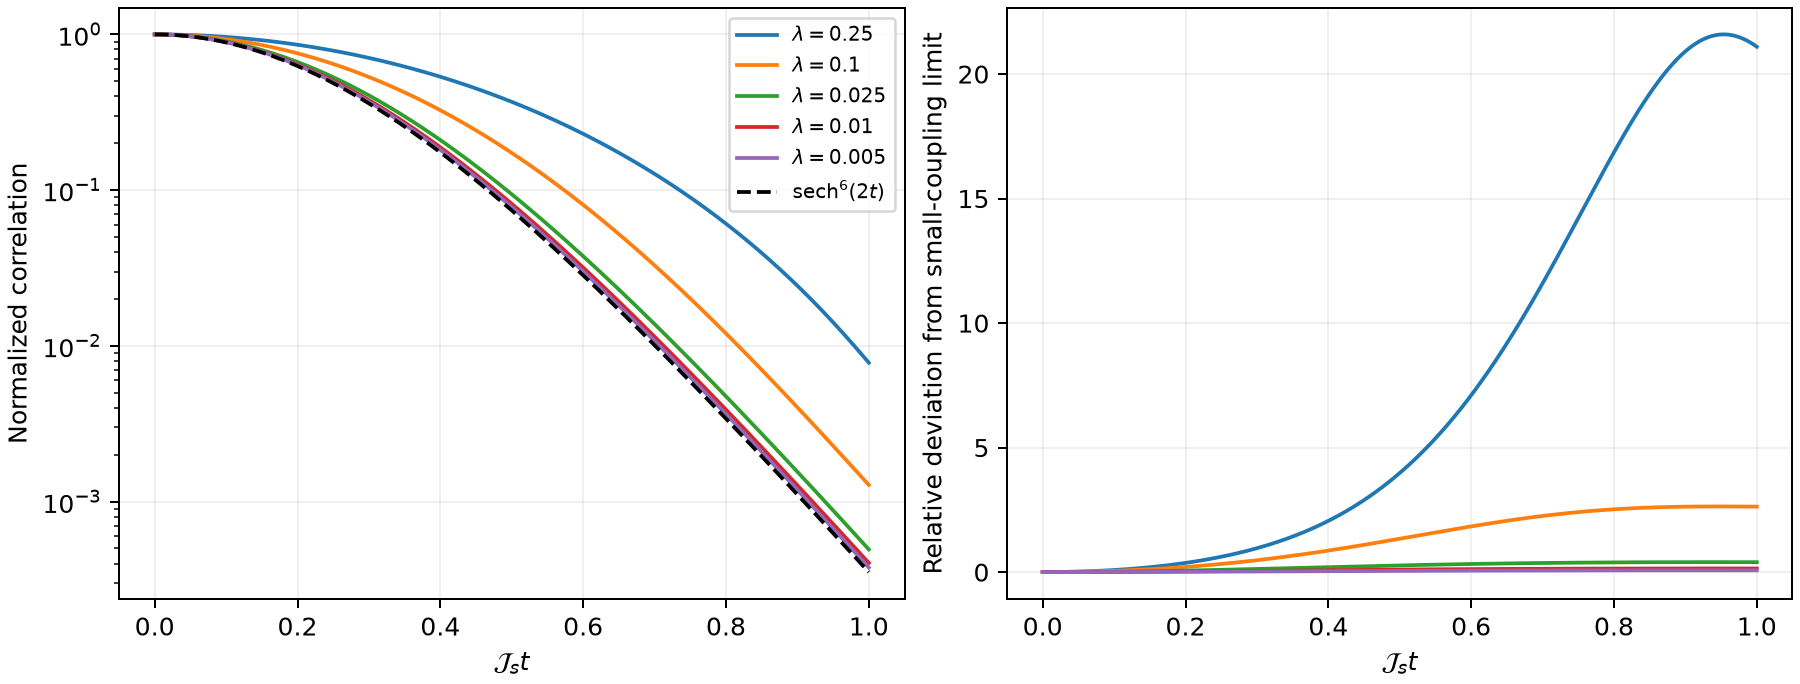
\includegraphics[width=\linewidth]{../../results/susskind-cubic-kernel/correlation.png}
\end{center}
The right panel retains relative finite-$\lambda$ differences.
Even at $\lambda=.005$, the difference at $\Js t=1$ is about
$7.09\%$; small absolute discrepancies at late times can otherwise
be misleading. No estimate uniform in growing time is inferred.

\newpage
\section{Validation, sources, and the next physical question}
The exact endpoint certificate covers 177 templates and 6234
distinct local matching words. Its independent integer-polynomial
verifier finds the same 176 vanishing templates and surviving
coefficients. The preceding stage's CAR identities and finite
marked-word tests are preserved unchanged.

The kernel was evaluated for
$\lambda=.25,.1,.025,.01,.005$ on $0\le\Js t\le1$.
Jacobi sizes were $33,52,138,302,574$, each compared to size
$L+16$. For $a=t_{\max}\|T_q\|$ and $L+1>a$, the shared first
$L$ Taylor terms imply the absolute truncation bound
\begin{equation}
 |C_R(t)-C_R^{(L)}(t)|
 \le \frac{4a^L}{L!}\frac{1}{1-a/(L+1)}<10^{-13}.
\end{equation}
This bounds truncation in exact arithmetic. Numerical eigenvalue
roundoff is tested by refinement, not included in an interval
certificate. At $\lambda=.25,.1$, independent Mehler quadratures
with 128 and 192 nodes reproduce the time values and moments
$\mu_0,\mu_2,\mu_4$; the largest Jacobi--Mehler absolute discrepancy
is below $4\times10^{-14}$. Full parameters, relative errors,
dependencies and hashes accompany the output.

\paragraph{What is borrowed and what is established here.}
The $q$-Hermite recurrence, probe strength density, and Mehler
kernel are established results \cite{BNR,TT}. The Gaussian
coupling-chaos operation defining $R$ is not identified blindly
with Hamiltonian $q$-Wick ordering. Hosomichi--Sato
\cite{HS}, Sec.~4, provide a useful precedent for proving composite
relations through local chord sums, but their degenerate
$d=-1/2$ fusion relation is a different construction. The new
step recorded here is the all-order two-insertion reduction for
the specified cubic derivative composite. We do not claim priority.

\paragraph{Next step.}
Complete the relation to the unprojected derivative family by
calculating the linear Gaussian chaos of $T_3$. Then study mixed
higher correlators of this $d=3$ channel and the existing $d=2$
singlet. Their mutual crossing rules and interactions have not
been established by a two-insertion proof. These provide concrete
new microscopic data for the Susskind program; spatial translation
and mass identification still require the bulk dictionary.
The full de Sitter duality remains an active research objective.

\begin{thebibliography}{9}
\bibitem{BNR} M. Berkooz, V. Narovlansky and H. Raj,
\emph{Complex Sachdev--Ye--Kitaev model in the double scaling limit},
\href{https://arxiv.org/html/2006.13983v2}{arXiv:2006.13983v2}, Sec.~7.
\bibitem{TT} J. Tall and S. Tomsovic,
\emph{Double-scaled bosonic and fermionic embedded ensembles,
complex SYK, and the dual Hilbert space},
\href{https://arxiv.org/html/2604.14522v2}{arXiv:2604.14522v2},
Secs.~3.1 and 4.1.
\bibitem{LS} H. W. Lin and D. Stanford,
\emph{A symmetry algebra in double-scaled SYK},
\href{https://arxiv.org/html/2307.15725v1}{arXiv:2307.15725v1}, Sec.~2.
\bibitem{HS} K. Hosomichi and M. Sato,
\emph{Degenerate chords in double-scaled SYK},
\href{https://arxiv.org/html/2512.01177v2}{arXiv:2512.01177v2},
Sec.~4, especially Eqs.~(4.19)--(4.26).
\end{thebibliography}
\end{document}
